%!TEX root = ../thesis.tex
%*******************************************************************************
%****************************** Second Chapter *********************************
%*******************************************************************************

\chapter{Modelos predictivos asociados a mutaciones puntuales en proteínas}

\ifpdf
    \graphicspath{{Chapter2/Figs/Raster/}{Chapter2/Figs/PDF/}{Chapter2/Figs/}}
\else
    \graphicspath{{Chapter2/Figs/Vector/}{Chapter2/Figs/}}
\fi

El análisis del efecto de mutaciones puntuales en proteínas, es una de las problemáticas más estudiadas en los últimos años. Los estudios se enfocan principalmente, en la evaluación de cambios en la estabilidad de la proteína mediante la variación de energía libre que la mutación provoca \cite{Schymkowitz2005,Pandurangan2017,rohl2004protein,Parthiban2006}. 

Diferentes modelos predictivos han sido desarrollados para poder predecir cambios de energía libre, en base a algoritmos de aprendizaje supervisado o mediante técnicas de minería de datos, y así, determinar el efecto de la mutación en set de proteínas de interés \cite{Quan2016,Capriotti2008,Broom2017,Khan2010,vaisman,Getov2016,Capriotti2005}. No obstante, en casos más específicos, se han desarrollado modelos para proteínas independientes, con el fin de asociar la mutación a un rasgo clínico, particularmente, enfocado a casos de cáncer \cite{article, Forbes2010}, cambios en termo estabilidad \cite{Tian2010}, propiedades geométricas \cite{Barenboim2008}, entre las principales.

Sin importar el uso o la respuesta de los modelos, es necesario construir set de datos con ejemplos etiquetados, es decir, cuya respuesta sea conocida para poder entrenar modelos basados en algoritmos de aprendizaje supervisado y así evaluar su desempeño. Los enfoques principales al desarrollo de descriptores se basan en propiedades fisicoquímicas y termodinámicas, así como también, el ambiente bajo el cual se encuentra la mutación \cite{Capriotti2005}, ya sea a partir de la información estructural o sólo considerando la secuencia lineal. Sin embargo, no son considerados, los componentes asociados a conceptos filogenéticos y la propensión a cambios de dicha mutación generando un gap entre ambos puntos de vista \cite{Olivera-Nappa2011}.

Dado a los modelos existentes y en vista a la necesidad de generar nuevos sistemas de predicción para mutaciones puntuales en proteínas, en respuesta al aumento considerable de reportes en los últimos años, se propone una nueva metodología para el diseño e implementación de modelos predictivos en mutaciones puntuales de proteínas.

Las mutaciones son descritas desde los puntos de vista estructural, termodinámico y filogenético. El desarrollo de los predictores es inspirados en el concepto de Meta Learning y es apoyado con técnicas estadísticas, tanto para la selección de modelos como para la evaluación de medidas de desempeño, entregando como resultado, un conjunto de modelos para las mutaciones puntuales reportadas unificados en un único meta modelo.

Esta metodología será aplicada para generar estimadores en diferentes proteínas con mutaciones reportadas con respuesta conocida, como por ejemplo: evaluando las diferencias de energía libre que provoca la mutación y clasificaciones para evaluar si la sustitución de residuos aumenta o disminuye la estabilidad. A su vez, se implementarán modelos de clasificación para determinar la propensión clínica en un conjunto de mutaciones conocidas relacionados con el gen \textit{p}VHL, responsable de la enfermedad von Hippel Lindau, con el fin de exponer la versatilidad de la metodología.

A continuación, se describen los principales conceptos relacionados a minería de datos y aprendizaje supervisado, seguido de algunas herramientas computacionales para el análisis de mutaciones y su relevancia en la de estabilidad de una proteína, continuando con la metodología propuesta, la caracterización de los diferentes set de datos a utilizar y resultados parciales obtenidos al aplicar esta metodología.

\section{Minería de datos}


Minería de datos es el proceso de descubrimiento de patrones en set de datos, involucrando métodos asociados a Machine Learning, Estadísticas y sistemas de bases de datos. \cite{hand2006data}. La minería de datos es un subcampo interdisciplinario de la informática, el cual tiene por objetivo general extraer información (a través de métodos inteligentes) de un conjunto de datos y transformar la información en una estructura comprensible para su uso posterior. \cite{fayyad1996knowledge, dunham2006data}. La minería de datos es el paso de análisis del proceso de \textit{descubrimiento de conocimiento en bases de datos}, o KDD. \cite{fayyad1996kdd}. Además del análisis en bruto de los datos, también incluye aspectos de manipulación de bases de datos y pre procesamiento de datos, evaluaciones de modelo e inferencia, métricas de interés, consideraciones de complejidad, post procesamiento de estructuras descubiertas, visualización y actualización de la información \cite{berry2004data}.

En la Figura \ref{intro1}, se exponen las principales ramas que componen la minería de datos y los diferentes procesos que se asocian a dichas ramas.

\begin{figure}[!h]
	
	\centering
	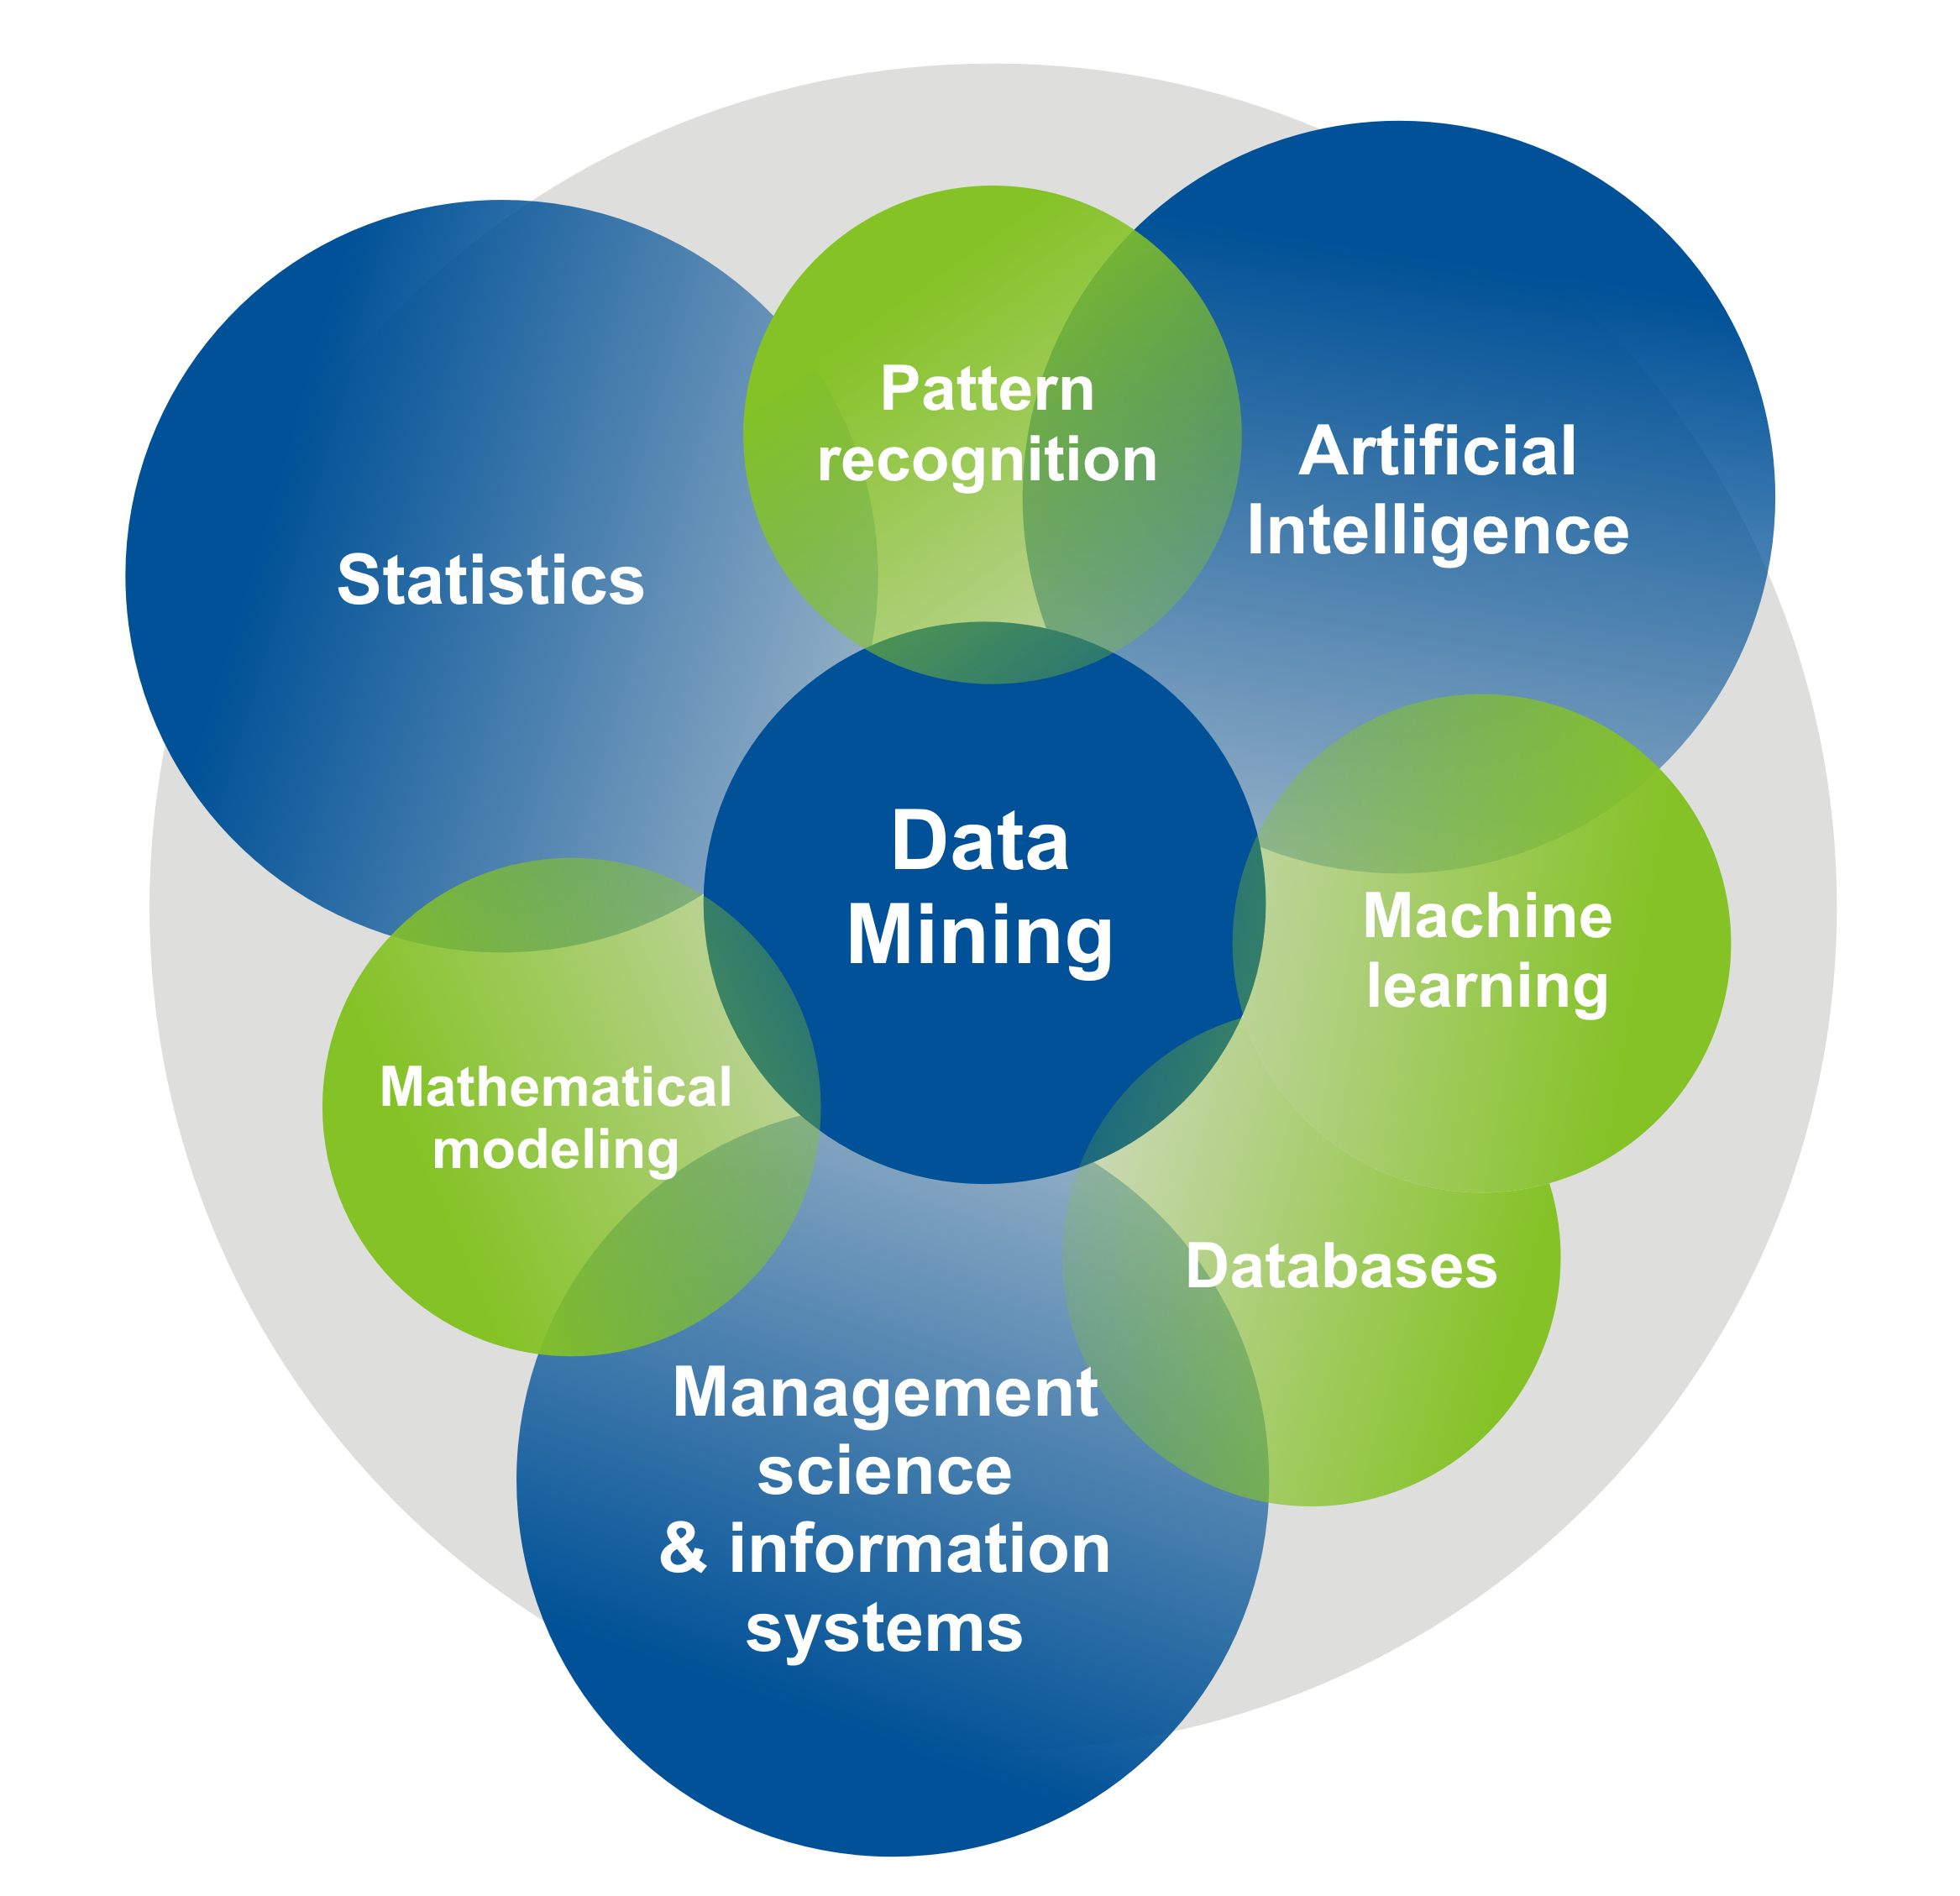
\includegraphics[scale=.4]{dataMining.jpg}
	\caption{Componentes en la minería de datos}
	\label{intro1}
\end{figure}

Son tres las principales áreas que abarca la minería de datos: Estadística, Inteligencia Artificial y Manipulación de sistemas de información. Por otro lado, son distintos procesos los que interactúan entre estas ramas, tales como: Modelamiento Matemático, reconocimiento de patrones, Sistemas de almacenamiento persistente y machine learning \cite{hand2006data}.

Cada área en particular tiene un objetivo general y diversos objetivos específicos. Sin embargo, estas áreas interactúan entre sí, con el fin de poder extraer patrones de información que generen conocimientos a partir de la data de procesada \cite{berry2004data}.

La minería de datos se utiliza en diferentes campos, tales como: genética y genómica \cite{Lee2008, Rebhan1998}, ingeniería de proteínas \cite{han2009research, 4548625, li2008fast}, comercio y negocios \cite{hofmann2013rapidminer}, sistemas de tránsito \cite{Ma2013}, optimizaciones en procesos industriales \cite{Chien2008, 8051033, 983448}, reconocimiento de patrones \cite{jain1988algorithms, fayyad1996data}, rasgos cuantificables en enfermedades \cite{Yoo2012, obenshain2004, LDuan} y más recientemente en áreas de dinámicas moleculares \cite{Chen2017, Yang:2005:GFM:1081870.1081962} y parámetros para la generación de pipe lines automatizados de simulaciones cuánticas en sistemas químicos \cite{MAO2004787, PhysRevLett.91.135503, Ramakrishnan2015}.

\section{Aprendizaje de Máquinas}

Aprendizaje de Máquina, es una rama de la inteligencia artificial que tiene por objetivo el desarrollo de técnicas que permitan a los computadores aprender, es decir, generalizar comportamientos a partir de una información no estructurada suministrada en forma de ejemplos \cite{michie1994machine}. Aplicándose en diferentes campos de investigación: motores de búsqueda \cite{cooley1997web}, diagnósticos médicos \cite{7912315,ABDELAZIZ2018117}, detección de fraude en el uso de tarjetas de crédito, bioinformática \cite{juanito}, reconocimiento de patrones en imágenes \cite{imageA} y textos \cite{netzer2011reading,alm2005emotions}, etc. 

Los algoritmos de aprendizaje pueden clasificarse en dos grandes grupos \cite{michie1994machine}:

\begin{itemize}
	
	\item \textbf{Supervisados}: se cumple un rol de predicción, clasificación, asignación, etc. a un conjunto de elementos con características similares, por lo que los datos de entrada son conocidos.
	
	\item \textbf{No Supervisados}: su objetivo es agrupar en conjuntos con características similares los elementos de entrada dado los valores de estos atributos, en base a la asociación de patrones característicos que representen sus comportamientos.
\end{itemize}

A continuación se describen en forma general, los algoritmos de aprendizaje supervisados utilizados para el desarrollo de la metodología, explicando los conceptos bajo los que se basan y cómo estos entrenan y se emplean para predecir o clasificar nuevos ejemplos.

\subsection{Algoritmos de aprendizaje supervisado}

Existen diferentes algoritmos de aprendizaje supervisado, los cuales pueden ser asociados a la clasificación de un elemento o la predicción de valores, dependiendo el tipo de respuesta existente en el conjunto de datos a estudiar. En el caso de respuestas con distribución continua, se trabajan con algoritmos de regresión, mientras que si la respuesta es binaria o multiclase y es representada por variables categóricas, los algoritmos se basan en clasificadores \cite{michie1994machine}.

A su vez, también se pueden dividir con respecto a la forma en que se trata el problema, existiendo algoritmos basados en cálculos de distancia entre ejemplos (K-Vecinos Cercanos), otros que consideran transformaciones vectoriales y aplicaciones de funciones de kernel (Máquina Soporte de Vectores), así como también el uso de las características como entorno espacial de decisión (Árboles y métodos de ensamble) y aquellos que utilizan redes neuronales y trabajan en torno a cajas negras, o métodos basados en regresiones lineales, sólo aplicados a modelos predictivos de variables continuas.

Cada uno de estos algoritmos es descrito a continuación, enfocándose tanto en el componente matemático asociado, así como también en las ventajas y usos posibles que estos puedan tener, con respecto al conjunto de datos a trabajar.

\subsection{K-Vecinos Cercanos}

Algoritmo de aprendizaje supervisado, el cual tiene por objetivo asociar un elemento a una clase en particular, dada la información de ejemplos de entrada que tengan asociadas características particulares, que puedan declararse como \textit{vecinos} del nuevo ejemplo a clasificar, siendo \textbf{k} el número de vecinos que se está dispuesto a utilizar para aplicar la clasificación \cite{6313426}. La mejor elección de \textbf{k} depende fundamentalmente de los datos; generalmente, valores grandes de \textbf{k} reducen el efecto de ruido en la clasificación, pero crean límites entre clases parecidas.

Con el fin de evaluar la cercanía de los ejemplos existentes contra el nuevo ejemplo a clasificar es necesario asociar ciertas medidas de distancia que permitan cuantificar esta cartacterística, para así poder comparar esta distancia y evaluar la cercanía para asociarle una clase a este nuevo ejemplo \cite{5408784}. La distancia a emplear para evaluar la cercanía puede ser: Euclidiana \cite{DANIELSSON1980227}, Manhattan \cite{PERLIBAKAS2004711}, coseno \cite{LIAO20155328}, Mahalanobis \cite{DEMAESSCHALCK20001}, entre las principales, las cuales son expuestas de manera general en la Tabla \ref{tab:tab-form-distance}.

% Please add the following required packages to your document preamble:
% \usepackage{longtable}
% Note: It may be necessary to compile the document several times to get a multi-page table to line up properly
\begin{longtable}[c]{|l|l|l|}
	\hline
	\multicolumn{1}{|c|}{\textbf{Distancia}} & \multicolumn{1}{c|}{\textbf{Fórmula}}                  & \multicolumn{1}{c|}{\textbf{Descripción}}                                                            \\ \hline
	\endfirsthead
	%
	\endhead
	%
	Euclideana                               & $D_{(X,Y)}\ =\ \sqrt{\sum_{i=1}^{l}(X_{i}-Y_{j})^{2}}$ & Se basa en una recta entre dos puntos                                                                \\ \hline
	Coseno                                   & $D_{(X,Y)}\ =\ \arccos(\frac{X^{T}Y}{||X||\ ||Y||})$   & \begin{tabular}[c]{@{}l@{}}Se basa en vectores y en el coseno del\\ ángulo que forman\end{tabular}   \\ \hline
	Manhattan                                & $D_{(X,Y)}\ =\ \sum_{i=1}{n} |X_{i}-Y_{i}|$            & Distancia en forma de zig-zag                                                                        \\ \hline
	Mahalanobis                              & $D_{(X,Y)}\ =\ \sqrt{(X-Y)^{T}S^{-1}(X-Y)}$            & \begin{tabular}[c]{@{}l@{}}Considera las correlaciones entre las\\ variables de estudio\end{tabular} \\ \hline
	\caption{Resumen tipos de distancias utilizadas en procesos de comparación de ejemplos
	}
	\label{tab:tab-form-distance}\\
\end{longtable}


K-Nearest Neighbors (KNN por su descripción en inglés), presenta algunos problemas, tales como: posibles errores al existir más de un elemento de distinta clase cercano al nuevo ejemplo a clasificar. Sin embargo, dicho error estimado es reducido \cite{6313426}.

Existen dos variaciones para la aplicación de KNN: aplicación basada en las distancias y aplicación basada en radios con respecto a puntos, la primera es mayormente usada. No obstante, en el caso de que los puntos no se encuentren uniformemente distribuidos es una mejor opción usar la segunda alternativa, siendo muy eficaz en problemas conocidos como \textit{la maldición de la dimensionalidad}. 

KNN utiliza el componente de peso \cite{TAN2005667}, es decir, valores asignados a puntos específicos para determinar si un elemento a clasificar es de una clase o no, normalmente se utilizan pesos uniformes, sin embargo, es posible asignar valores de tal manera que al momento de realizar la votación puntos más cercanos en base a distancias presenten más peso que otros.

Se han implementando diversos algoritmos a la hora de aplicar la técnica de KNN, los cuales tienen relación con el coste computacional que presentan, dentro de estos se encuentran: Brute Force, K-D Tree y Ball Tree \cite{pedregosa2011scikit}.

Este algoritmo de aprendizaje supervisado, puede ser utilizado tanto para el entrenamiento de modelos de clasificación (respuestas categóricas) y de regresión (respuestas continuas).

\subsection{Naive Bayes}

Naive Bayes es un conjunto de algoritmos de aprendizaje supervisados basados en la aplicación del teorema de Bayes con la suposición "ingenua" de independencia entre cada par de características \cite{zhang2004optimality}. Dada una variable de clase $y$ y un vector de característica dependientes de la forma $x_1,..., x_n$, el teorema de Bayes establece la siguiente relación:

\begin{center}
	$P(y \mid x_1, \dots, x_n) = \frac{P(y) P(x_1, \dots x_n \mid y)} {P(x_1, \dots, x_n)}
	$
\end{center}

Utilizando la suposición ingenua de independencia de características, se tiene que:

\begin{center}
	$P(x_i | y, x_1, \dots, x_{i-1}, x_{i+1}, \dots, x_n) = P(x_i | y)$
\end{center}

Para todo $i$, esta relación se simplifica a:

\begin{center}
	$P(y \mid x_1, \dots, x_n) = \frac{P(y) \prod_{i=1}^{n} P(x_i \mid y)} {P(x_1, \dots, x_n)}$
\end{center}

Dado que $P(x_1, \dots, x_n)$ es constante dada la entrada, se puede utilizar la siguiente regla de clasificación:

\begin{center}
	$P(y \mid x_1, \dots, x_n) \propto P(y) \prod_{i=1}^{n} P(x_i \mid y)$
	
\end{center}

\begin{center}
	$\Downarrow$ 
\end{center}
\begin{center}
	$\hat{y} = \arg\max_y P(y) \prod_{i=1}^{n} P(x_i \mid y),$
\end{center}

A pesar de sus supuestos aparentemente simplificados, los clasificadores de Naive Bayes han funcionado bastante bien en muchas situaciones del mundo real, la famosa clasificación de documentos y el filtrado de spam son ejemplos de ello \cite{10.1007/BFb0026666, Chen2009, metsis2006spam}. Requieren una pequeña cantidad de datos de entrenamiento para estimar los parámetros necesarios. Pueden ser extremadamente rápido en comparación con métodos más sofisticados. El desacoplamiento de las distribuciones de las características condicionales de clase significa que cada distribución se puede estimar de forma independiente como una distribución unidimensional. Esto a su vez ayuda a aliviar los problemas derivados de la dimensionalidad. 

Existen distintos tipos de clasificadores de Naive Bayes, diferenciándose entre sí en la función de distribución de probabilidad que utilizan \cite{metsis2006spam,john1995estimating,manning2010introduction}, dentro de los que se encuentran:

\begin{itemize}
	
	\item \textbf{Gaussian Naive Bayes.}
	
	\begin{center}
		$P(x_i \mid y) = \frac{1}{\sqrt{2\pi\sigma^2_y}} \exp\left(-\frac{(x_i - \mu_y)^2}{2\sigma^2_y}\right)$
	\end{center}
	
	\item \textbf{Multinomial Naive Bayes.}
	
	La distribución se parametriza por el vector $\theta_y = (\theta_{y1},\ldots,\theta_{yn})$ para cada clase $y$, donde $n$ es el número de características y $\theta_{y1}$ es la probabilidad $P(x_i \mid y)$ de que la característica $i$ aparezca en una muestra que pertence a la clase $y$.
	
	Cada $\theta_y$ es estimado por:
	
	\begin{center}
		
		$\hat{\theta}_{yi} = \frac{ N_{yi} + \alpha}{N_y + \alpha n}$		
	\end{center}
	
	Donde $N_{yi} = \sum_{x \in T} x_i$ es el número  de veces que aparece la característica $i$ en la muestra de clase $y$ en el set de entrenamiento $T$ y $N_{y} = \sum_{i=1}^{|T|} N_{yi}$ representa el total de todas las características para la clase.
	
	\item \textbf{Bernoulli Naive Bayes.}
	
	\begin{center}
		$P(x_i \mid y) = P(i \mid y) x_i + (1 - P(i \mid y)) (1 - x_i)$
	\end{center}
	
\end{itemize}

\subsection{Árboles de Decisión}

Se define árbol de  decisión como un modelo de predicción utilizado en el ámbito de la inteligencia artificial, en el cual,  dado un conjunto de datos se fabrican diagramas de construcciones lógicas, muy similares a los sistemas de predicción basados en reglas, que sirven para representar y categorizar una serie de condiciones que ocurren de forma sucesiva, para la resolución de un problema.  Aprendizaje basado en árboles de decisión es un método comúnmente utilizado en la minería de datos, cuyo objetivo consiste en desarrollar un modelo de predicción para el valor de una variable de destino en función de diversas variables de entrada \cite{freund1999alternating}.

El aprendizaje basado en árboles de decisión utiliza un árbol como un modelo predictivo que mapea las observaciones de las características que presenta un elemento. En estas estructuras de árbol, las hojas representan etiquetas de conjuntos ya clasificados, los nodos, a su vez, nombres o identificadores de los atributos y las ramas representan posibles valores para dichos atributos, a modo de ejemplo, se expone en la Figura \ref{arboles}, una representación de un posible árbol, el cual fue desarrollado para entrenar modelos de clasificación utilizando el set de datos iris \cite{fisher1936use}.

\begin{figure}[!h]
	
	\centering
	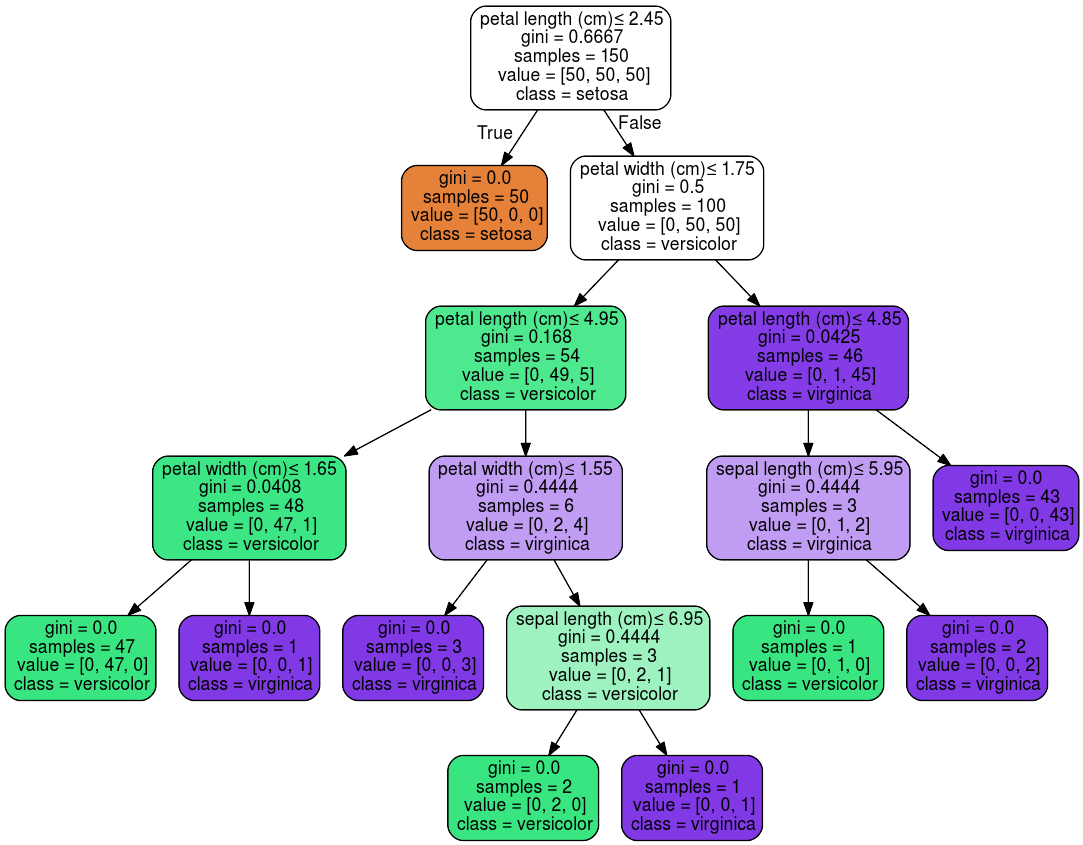
\includegraphics[scale=.4]{iris.png}
	\caption{Estructura de árbol para modelo de clasificación de set de datos iris.}
	\label{arboles}
\end{figure}

Un árbol de decisión es una representación simple para clasificar ejemplos, el aprendizaje basado en esta metodología es una de las técnicas más eficientes para la clasificación supervisada. Donde cada ejemplo consta de atributos con valores discretos dentro de un dominio de conjunto finito, y existe un sólo término final denominado clasificación. En un árbol de decisión, cada elemento del dominio de la clasificación se llama clase, cada nodo interno (no hoja) está etiquetado con una función de entrada, las ramas procedentes de un nodo etiquetado con una característica están asociados con cada uno de los posibles valores de la característica. Cada hoja del árbol se marca con una clase o una distribución de probabilidad sobre las clases \cite{bhargava2013decision}.

Un árbol puede ser entrenado mediante el fraccionamiento del conjunto inicial en subconjuntos basados en una prueba de valor de atributo. Este proceso se repite en cada subconjunto derivado de una manera recursiva llamada particionamiento recursivo. La recursividad termina cuando el subconjunto en un nodo tienen todos el mismo valor de la variable objetivo, o cuando la partición ya no agrega valor a las predicciones.

Para cada división, es necesario el uso de una función que entregue una medida de impureza en cada división, esto con el objetivo de seleccionar la mejor partición para un atributo dado, la elección de dicho atributo se basa en el objetivo de separar de mejor manera los ejemplos. 

La selección de los atributos se basa en qué atributo al momento de clasificar genera nodos más puros, para ello se utiliza una función de ganancia de información, la cual representa la ganancia  obtenida a partir de una división de los ejemplos de entrenamiento \cite{breiman2017classification}. 

Existen diferentes tipos de algoritmos basados en árboles de decisión, los cuales se exponen brevemente en la Tabla resumen .

Una definición matemática, tanto del proceso de clasificación o regresión y cómo son los criterios de selección de atributos es expuesta a continuación.

Sea $x_{i} \in R^{n}$ los vectores de entrenamiento del conjunto de datos y sea $y \in R^l$ el vector de respuestas asociadas a cada ejemplo, un árbol de decisión divide el espacio de forma recursiva, de manera que las muestras con las mismas etiquetas se agrupan.

Cada nodo $m$ puede ser representado por $Q$ y sea $\theta = (j, t_{m})$ la división candidata para un atributo $j$ y un umbral $t_{m}$, se definen las particiones $Q_{left}(\theta)$ y $Q_{rigth}(\theta)$ tal que:

\begin{align}
	\begin{aligned}
		Q_{left}(\theta) = {(x, y) | x_j <= t_m}\\Q_{right}(\theta) = Q \setminus Q_{left}(\theta)
	\end{aligned}
\end{align}
 

Asociado a las divisiones, se tiene que, cada nodo generado se mide con respecto a la impureza de éste, la cual puede ser representada por una función $H()$ y a la ganancia de información que genera la división $G(Q, \theta)$, la cual se estima como:

\begin{center}
	$G(Q, \theta) = \frac{n_{left}}{N_m} H(Q_{left}(\theta))
+ \frac{n_{right}}{N_m} H(Q_{right}(\theta)$
\end{center}

Los descriptores se seleccionan con respecto a aquel que minimice la impureza de los nodos:

\begin{center}
	$\theta^* = \operatorname{argmin}_\theta  G(Q, \theta)$
\end{center}

Finalmente, se tiene que para los subconjuntos $Q_{left}(\theta^*)$ y $Q_{rigth}(\theta^*)$ la profundidad máxima se alcanza si:

\begin{itemize}
	
	\item $N_{m} < min_{samples}$ 
	
	\item $N_{m} = 1$
\end{itemize}

Con $N_{m}$ representando el número de nodos $m$.

Los criterios de clasificación se basan en la proporción de las clases según sus observaciones y en la función de impureza que es posible utilizar.

Si el vector de respuestas, es asociado a variables categóricas y toma valores entre $0,1,\cdots,k-1$ para un nodo $m$, representando una región $R_{m}$ con $N_{m}$ ejemplos, se tiene que la proporción  de observaciones de clase $k$ en un nodo $m$ puede definirse como:

\begin{center}
	$p_{mk} = 1/ N_m \sum_{x_i \in R_m} I(y_i = k)$
\end{center}

Con respecto a las diferentes funciones de impureza $H()$ que pueden ser utilizadas se tienen las siguientes, descritas en la Tabla \ref{tab:tab-form-impureza}. 

% Please add the following required packages to your document preamble:
% \usepackage{longtable}
% Note: It may be necessary to compile the document several times to get a multi-page table to line up properly
\begin{longtable}[c]{|l|l|}
	\hline
	\multicolumn{1}{|c|}{\textbf{Función}} & \multicolumn{1}{c|}{\textbf{Fórmula}}   \\ \hline
	\endfirsthead
	%
	\endhead
	%
	Gini                                   & $H(X_m) = \sum_k p_{mk} (1 - p_{mk})$   \\ \hline
	Entropía                               & $H(X_m) = - \sum_k p_{mk} \log(p_{mk})$ \\ \hline
	Misclassification                      & $H(X_m) = 1 - \max(p_{mk})$             \\ \hline
	\caption{Tipos de medidas de impureza que pueden ser utilizadas en árboles de decisión para modelos de clasificación.
	}
	\label{tab:tab-form-impureza}\\
\end{longtable} 

Siendo $X_{m}$ datos de entrenamiento en el nodo $m$.

A la hora de entrenar modelos de regresión, es decir, con respuestas con distribución continua, se tiene que para el nodo $m$, el cual representa una región $R_{m}$ con observaciones $N_{m}$, los criterios comunes para minimizar errores en futuras divisiones son el Error cuadrático medio y el Error absoluto medio, quienes minimizan el error tipo II y el error tipo I, respectivamente.

Estos se pueden definir como:

\begin{itemize}
	
	\item \textbf{Error cuadrático medio}: 
	
	\begin{align}\begin{aligned}\bar{y}_m = \frac{1}{N_m} \sum_{i \in N_m} y_i\\H(X_m) = \frac{1}{N_m} \sum_{i \in N_m} (y_i - \bar{y}_m)^2\end{aligned}\end{align}
	
	\item \textbf{Error absoluto medio}: 
	
	\begin{align}\begin{aligned}\bar{y}_m = \frac{1}{N_m} \sum_{i \in N_m} y_i\\H(X_m) = \frac{1}{N_m} \sum_{i \in N_m} |y_i - \bar{y}_m|\end{aligned}\end{align}
\end{itemize}


\section{Herramientas computacionales asociadas a evaluación de mutaciones}

Las herramientas computacionales asociadas a la evaluación de mutaciones puntuales se centran principalmente en el análisis de cómo ésta afecta a la estabilidad o la predicción de energía libre asociada a los residuos involucrados en la mutación. Sin embargo, a pesar de que el objetivo es el mismo, se enfocan en diferentes puntos de vista para abordar la problemática, tanto a nivel de entrenamiento de modelos, cómo manipulación de set de datos, así como las técnicas utilizadas para la predicción de los cambios de energía libre.

A continuación, se exponen algunas herramientas relacionadas con el estudio de estabilidad de proteínas, las cuales se aplicarán como métodos de comparación para los resultados obtenidos aplicando la metodología propuesta.

\subsection{FoldX}

FoldX es una herramienta computacional, que implementa un campo de fuerza empírico, desarrollado para la evaluación eficiente del efecto de las mutaciones sobre la estabilidad, el plegamiento y la dinámica de las proteínas y los ácidos nucleicos \cite{Schymkowitz2005}. Se basa principalmente en el cálculo de energía libre a partir de estructuras 3D de macromoléculas. Sin embargo, permite además, estimar las posiciones de los protones y los puentes de hidrógeno. 

La energía libre, es calculada utilizando la siguiente expresión matemática de aportes energéticos:


$\Delta G=Wvdw \cdot \Delta Gvdw+WsolvH \cdot \Delta GsolvH+WsolvP \cdot \Delta GsolvP+ \Delta Gwb+ \Delta Ghbond+ \Delta Gel+ \Delta GKon+Wmc \cdot T \cdot \Delta Smc+Wsc \cdot T \cdot \Delta Ssc$

Los componentes se definen a continuación.

\begin{itemize}
	
	\item $\Delta Gvdw$ es la suma de las contribuciones de van der Waals de todos los átomo con respecto a la interacción con el solvente.
	
	\item $\Delta GsolvH$ y $\Delta GsolvP$ son las diferencias en energía de solvatación para grupos apolares y polares respectivamente, cuando estos cambian desde el estado no plegado a plegado.
	
	\item $\Delta Ghbond$ es la diferencia de energía libre entre la formación de un enlace de hidrógeno intra-molecular y uno inter-molecular.
	
	\item $\Delta Gwb$ es la energía libre de estabilización adicional proporcionada por una molécula de agua que hace más de un enlace de hidrógeno a la proteína que no se puede tener en cuenta con aproximaciones de solventes no explícitas \cite{petukhov1999local}. 
	
	\item $\Delta Gel$ es la contribución electrostática de los grupos cargados, incluyendo las hélices dipolo. 
	
	\item $\Delta Smc$ es el costo de la entropía de fijar el back-bone en el estado plegado; este término depende de la tendencia intrínseca de un aminoácido particular a adoptar ciertos ángulos diedros \cite{munoz1996local, munoz1995hydrophobic}. 
	
	\item $\Delta Ssc$ es el costo de entropía de fijar una cadena lateral en una conformación particular \cite{abagyan1994biased}. 
	
	\item Si la estimación se desarrolla sobre proteínas oligoméricas o complejos de proteína, se adicionan dos términos a la contribución energética: $\Delta Gkon$ que refleja el efecto de las interacciones electrostáticas en la constante de asociación $kon$ (esto se aplica solo a las energías de enlace de la subunidad) \cite{vijayakumar1998electrostatic} y $\Delta Str$ que es la pérdida de entropía traslacional y rotacional que se deriva de la formación del complejo. Este último término se cancela cuando observamos el efecto de mutaciones puntuales en complejos. 
	
	\item Los valores de energía de $\Delta Gvdw$, $\Delta GsolvH$, $\Delta GsolvP$ y $\Delta Ghbond$ atribuidos a cada tipo de átomo se han derivado de un conjunto de datos experimentales, y $\Delta Smc$ y $\Delta Smc$ han sido considerados desde estimaciones teóricas. 
	
	\item Los términos $Wvdw$, $WsolvH$, $WsolvP$, $Wmc$ y $Wsc$ corresponden a los factores de ponderación aplicados a los términos de energía bruta. Todos son 1, excepto por la contribución de van der Waals que es de 0.33 (las contribuciones de van der Waals se derivan de la transferencia de energía de vapor a agua, mientras que en la proteína vamos de solvente a proteína).
	
\end{itemize}

Como entrada principal, recibe una estructura PDB\footnote{Protein Data Bank. Formato para la exposición de macromoléculas u estructuras en torno a coordenadas espaciales, obtenidas desde una cristalografía de rayos X, resnonancia magnética nuclear, o a través de modelos computacionales.} y dentro de los resultados más relevantes, se encuentran los cálculos de energía libre.

Ha sido usada en diferentes investigaciones, incluyendo el análisis de mutaciones puntuales aplicados a ingeniería de proteínas \cite{BU201825, Alibes2010}, evaluación de mutaciones en genomas \cite{Sanchez2008}, análisis de termoestabilidad \cite{Bu2018, 10.1093/protein/gzv004}, interacciones proteínas-DNA \cite{NADRA20113}, entre las principales, razón por la cual, es considerada como una herramienta común a la hora de la evaluación de mutaciones y un referente para comparar resultados de nuevas herramientas o métodos computacionales.

\subsection{I-Mutant}

I-Mutant, es una familia de software basados en algoritmos de aprendizaje supervisado para la predicción automática de estabilidad de proteínas ante cambios de residuos o sustituciones expresadas en mutaciones puntuales \cite{capriotti2005mutant2}, las cuales se reflejan en los cambios de energía libre. Emplea como algoritmo para entrenamiento de modelos, Support Vector Machine (SVM), permitiendo la evaluación de las mutaciones desde la secuencia lineal de proteína o a su vez desde la estructura 3D en formato PDB.

El método fue entrenado y testeado desde la base de datos ProTherm \cite{Bava2004}, la cual representa el mayor repositorio de experimentos termodinámicos con respuestas en energía libre basados en cambios de estabilidad de la proteína para mutaciones, en diferentes condiciones. 

Actualmente  I-Mutant permite la clasificación de la estabilidad de la mutación y a su vez facilita la predicción de los cambios de energía libre $\Delta \Delta G$. Las medidas de desempeño se diferencian dependiendo del uso de I-Mutant y del tipo de set de datos. Si se trabaja con datos de secuencias lineales presenta una accuracy de un 77\% y un coeficiente de relación de un 0.62 con un error asociado de 1.45 kcal/mol. Para el caso en que los datos procedan de información estructural, los desempeños mejoran de manera no significativa, obteniendo una accuracy de un 80\% y un coeficiente de relación de un 0.71 con un error asociado de 1.30 kcal/mol.

Si bien, es uno de los métodos más utilizados, el hecho de utilizar Support Vector Machine como algoritmo de aprendizaje supervisado para el entrenamiento de modelos, es un punto limitante a la hora de utilizar set de datos altamente no lineales, dado a que el algoritmo sólo traza hiperplanos y transforma los elementos aplicando funciones de kernel, con el fin de maximizar la varianza. Esto podría provocar sobre ajuste o generar bajos desempeños.

\subsection{CUPSAT}

CUPSAT (Cologne University Protein Stability Analysis Tool) es una herramienta web para analizar y predecir la estabilidad de la proteína frente a cambios o sustituciones puntuales de residuos. La herramienta utiliza información estructural específica de los átomos participantes en la mutación, tales como: ángulos de torsión y potenciales de energía, con el fin de predecir los cambios en diferencia de energía que representa la sustitución, expresados en forma de $\Delta \Delta G$ \cite{Parthiban2006}. 

Como requisitos para su uso, es necesario la estructura en formato PDB y la posición del residuo a ser mutado. Como resultado, entrega información sobre el sitio de la mutación, principalmente accesibilidad al solvente, estructura secundaria y ángulos de torsión. Además, entrega información detallada sobre las 19 posibles mutaciones para el residuo objetivo.

La herramienta fue testeada utilizado 1538 mutaciones desde denaturaciones térmicas y 1603 denaturaciones aplicando técnicas químicas. Presentado un desempeño mayor al 80\% de accuracy.

Esta herramienta no aplica algoritmos de aprendizaje supervisado y se basa principalmente en el uso de técnicas asociadas a bioinformática estructural, para poder evaluar los cambios producidos por las sustituciones, además, permite analizar un espectro amplio de elementos dado a que, facilita el análisis de las 19 posibilidades de residuos, permitiendo hacer una evaluación de cuáles podrían ser sustituciones favorables y cuales no. El desempeño se obtiene al comparar los valores estimados por la herramienta contra resultados reportados en base de datos ProTherm \cite{Bava2004}.


\subsection{MultiMutate}


\subsection{Herramientas necesarias para la caracterización de los set de datos}

Adicional a las herramientas expuestas, se hace una descripción breve de SDM \cite{Pandurangan2017} y MOSST \cite{Olivera-Nappa2011}, las cuales serán utilizadas a lo largo de la metodología con el fin de poder caracterizar las mutaciones desde los puntos de vista termodinámico (aplicando SDM) y filogenético (por medio de MOSST).

\subsubsection{SDM}

\subsubsection{MOSST}

\section{Hipótesis}

En base a las herramientas existentes y en vista del aumento considerable de datos asociados a mutaciones en proteínas y el conocimiento de las respuestas que éstas generan, se evidencia la necesidad del desarrollo de herramientas computacionales o nuevos modelos de clasificación o regresión que faciliten el entrenamiento de proteínas singulares y la evaluación de sus mutaciones puntuales, con el fin de poder evaluar nuevos ejemplos y cuáles serían los efectos de estos, sin tener que recurrir en grandes costos económicos y tiempos de espera. 

Dado esto se propone la siguiente hipótesis.\\

\textit{Es posible utilizar técnicas de Meta Learning y algoritmos de aprendizaje supervisado para la generación de modelos de clasificación o regresión de mutaciones puntuales descritas a partir de sus propiedades termodinámicas y filogenéticas?}\\

Además de la hipótesis central surgen interrogantes como.

\begin{itemize}
	
	\item Es posible utilizar estos nuevos modelos como herramientas para diagnóstico médico?
	\item Cómo se evalúan la robustez y la generalización de estos modelos, serán capaces de adaptarse a nuevos ejemplos?
	\item Es factible el desarrollo de una herramienta computacional que permita entrenar diferentes set de datos y que facilite la clasificación de nuevos ejemplos?
	
\end{itemize}

\section{Objetivos}

En base a la hipótesis planteada y a las preguntas adicionales expuestas, se exponen a continuación el objetivo general y los objetivos específicos.

\subsection{Objetivo general}

Diseñar e implementar estrategias inspiradas en Meta Learning para la implementación de modelos de clasificación y regresión asociado a mutaciones puntuales en proteínas de interés basados en descriptores termodinámicos, estructurales y filogenéticos.

\subsection{Objetivos específicos}

Dentro de los objetivos específicos se encuentran los siguientes.

\begin{enumerate}
	
	\item Preparar y describir, por medio de propiedades termodinámicas, estructurales y filogenéticas, set de datos de mutaciones puntuales de proteínas con respuesta conocida expuestos en bibliografía o bases de datos reconocidas.
	
	\item Implementar y evaluar metodología de meta learning para el diseño de meta modelos de clasificación y regresión de mutaciones puntuales aplicados a set de datos de proteínas generadas.
	
	\item Diseñar e implementar herramienta computacional que permita el entrenamiento de set de datos y el uso de meta modelos para la evaluación de nuevos ejemplos.
	
	\item Testear y evaluar comportamiento de la herramienta y los meta modelos en base a sistemas de datos que involucren mutaciones en proteínas con respuesta conocida.
	
	\item Implementar modelos de clasificación para la relevancia clínica de mutaciones puntuales en proteína pVHL, asociada a la enfermedad von Hippel Lindau. 
	
\end{enumerate}

\section{Metodología propuesta}

Con el fin de poder responder a la hipótesis planteada y dar solución a los objetivos impuestos, se propone una metodología general, en la cual se consideran diferentes estrategias, implementaciones y evaluación de modelos. A continuación se explica la metodología propuesta y los componentes principales de ésta.

\subsection{Preparación de set de datos}

La preparación del set de datos consiste en obtener data para poder entrenar los modelos  predictivos, la data se asocia a información de mutaciones en proteínas y la respuesta que ésta genera. En la Figura \ref{C2:M1} se expone un esquema general con los pasos desarrollados para la preparación del set de datos.

\begin{figure}[!h]
	\centering
	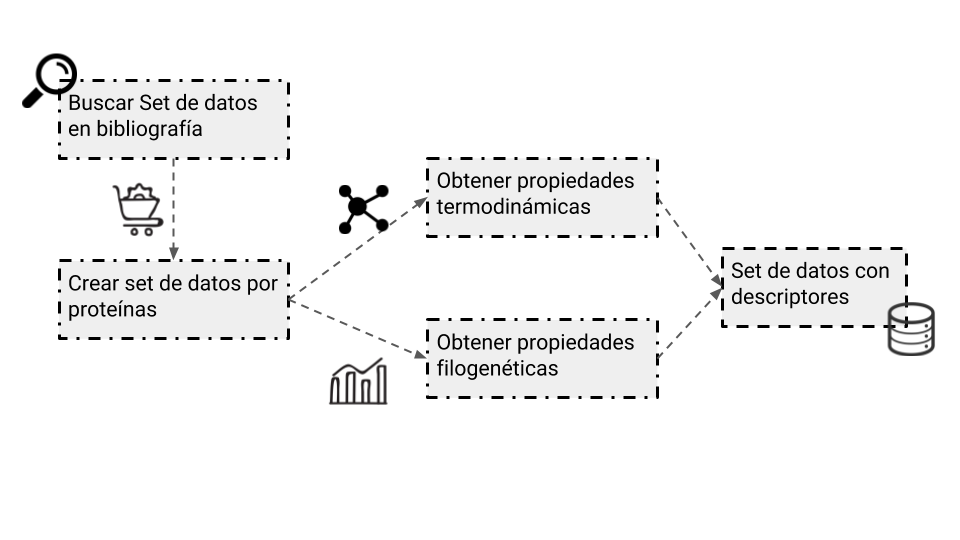
\includegraphics[scale=.4]{m1.png}
	\caption{Esquema representativo asociado al proceso de generación de set de datos de mutaciones puntuales en proteínas.}
	\label{C2:M1}
\end{figure}

Tal como se expone en la Figura \ref{C2:M1}, los set de datos se buscan en la bibliografía, a partir de modelos desarrollados previamente, bases de datos en la literatura, etc. El objetivo fundamental, es encontrar proteínas con mutaciones puntuales cuyo efecto sea conocido, dicha respuesta puede ser categórica, es decir, asociada al diseño e implementación de modelos de clasificación o continua y se aplica para modelos de regresión. 

En una segunda instancia, a partir de la data recolectada ésta se procesa con el fin de poder obtener set de datos de proteínas individuales con una cantidad de ejemplos considerables que permitan el diseño de modelos válidos, para ello, fueron implementados scripts bajo el lenguaje de programación Python con el fin de recuperar las proteínas, obtener la información y generar la data de manera individual, además, eliminar ejemplos ambiguos. Es decir, filas con los mismos valores pero cuya columna de respuesta fuese diferente. 

A partir de esto se forman $n$ set de datos asociados a $n$ proteínas, cada uno con $m$ ejemplos y cuyos descriptores consisten en el residuo original, posición en proteína, residuo mutado y la respuesta asociada. El desbalance de clases se analiza con respecto a las posibles categorías existentes en la respuesta y el porcentaje de representatividad que éstas poseen en la muestra. Se considera que el set de datos exhibe este comportamiento cuando presentan las características expuestas en la sección \textbf{CITAR PARTE ANTERIOR}. En este caso, los ejemplos se tratan con SMOTE (Synthetic Minority Oversampling Technique) \cite{chawla2002smote}

Posteriormente se aplican las herramientas SDM \cite{Pandurangan2017} y MOSST \cite{Olivera-Nappa2011} con el fin de obtener los descriptores asociados a las propiedades termodinámicas y filogenéticas. Para ello, scripts Python son desarrollados para consumir los servicios de dichas herramientas y registrar los resultados obtenidos, formando así, set de datos con los descriptores planteados en los objetivos iniciales. Un punto importante a destacar, es que el uso de SDM implica que las proteínas a trabajar, deben presentar una estructura 3D reportada en el Protein Data Bank \cite{berman2000protein} o al menos poseer un modelo representativo y validado. Esto es debido a que se utilizan informaciones de coordenadas para la estimación del efecto de la mutación, minimizaciones energéticas y estabilización de la mutante.

Ya con los descriptores formados, las características asociadas a variables categóricas son codificadas. Si la totalidad de posibles categorías supera el 20\% del total de características en el set de datos, se aplica Ordinal Encoder, en caso contrario, One Hot Encoder \cite{pedregosa2011scikit}. Ordinal Encoder consiste en la transformación de variables categóricas en arreglos de números enteros con valores desde $0,...,n-1$ para $n$ posibles categorías. Por otro lado, One Hot Encoder, consiste en agregar tantas columnas como posibles categorías existan en el set de datos completadas mediante binarización de elementos (0 si la característica no se presencia, 1 en caso contrario).

Es importante mencionar que las respuestas asociadas a las mutaciones pueden ser del tipo continuo o categórico, lo cual implica que tanto los modelos como las métricas varían. No obstante, se aplica la metodología indistintamente, con el fin de demostrar la robustez del método y la eficacia de éste sin importar el tipo de modelo que se éste entrenando.

\subsection{Implementación de meta modelos de clasificación/regresión}

La implementación de meta modelos consiste en la obtención de un grupo de estimadores que en conjunto, permiten clasificar o predecir nuevos ejemplos. Para ello, se diseña e implementa una metodología inspirada en Sistemas de Meta Learning y aplicando técnicas estadísticas para la evaluación del desempeño y el uso del meta modelo con nuevos ejemplos.

En la Figura \ref{C2:M2}, se exponen las etapas asociadas a la implementación de meta modelos, contemplando desde la fase de entrenamiento de los modelos hasta la unión en meta clasificadores (Paper en redacción). Cada una de las etapas contempla un conjunto de scripts implementados en lenguaje de programación Python y empleando la librería Scikit-Learn para el entrenamiento y evaluación de los clasificadores o predictores \cite{pedregosa2011scikit}, así como Numpy para el uso de módulos estadísticos \cite{doi:10.1109/MCSE.2011.37}.


\begin{figure}[!h]
	\centering
	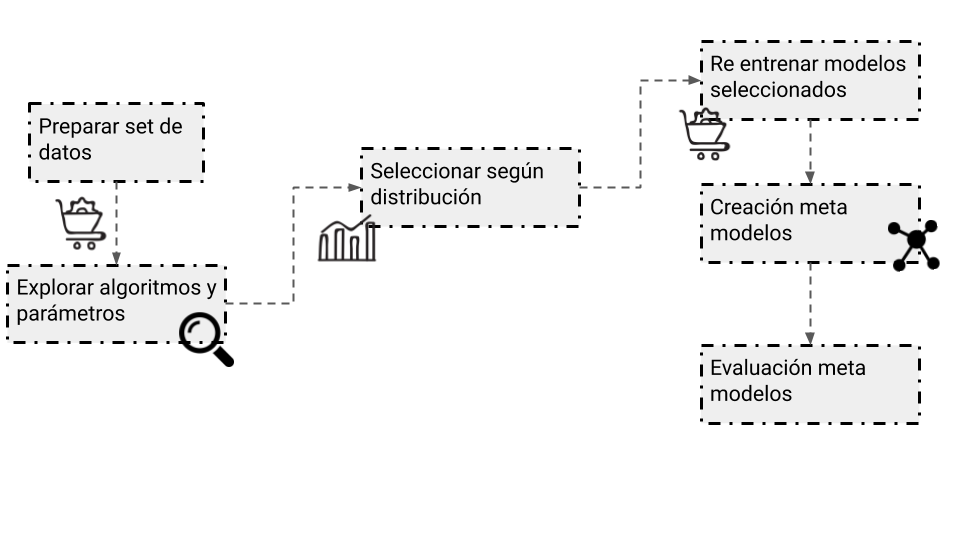
\includegraphics[scale=.4]{m2.png}
	\caption{Esquema representativo asociado al proceso de creación de meta modelos utilizando Meta Learning System Tools.}
	\label{C2:M2}
\end{figure}

Tal como se observa en la Figura \ref{C2:M2}, es posible identificar etapas claves en el proceso: Exploración de modelos, Selección y Generación de los meta clasificadores/predictores, junto con su evaluación. Cada una de estas etapas se exponen a continuación.

\subsubsection{Exploración de modelos}

La exploración de modelos o estimadores, se basa en la aplicación de diferentes algoritmos de aprendizaje supervisado con variaciones en sus parámetros de configuración inicial. La utilización de los algoritmos, depende principalmente del tipo de respuesta que presente el set de datos, es decir, si es continua o categórica. No obstante, a modo resumen, en la Tabla \ref{cap2:tab1} se exponen los algoritmos utilizados, el caso en el que se usan y los parámetros que se varían junto con el total de iteraciones posibles para cada elemento:

\begin{longtable}[c]{llll|l|l|}
	\hline
	\multicolumn{6}{|c|}{\textbf{Algoritmos y parámetros empleados en la etapa de Exploración en MLSTools}}                                                                                                                                                                                                                                                                                               \\ \hline
	\endfirsthead
	%
	\endhead
	%
	\multicolumn{1}{|l|}{\textbf{\#}} & \multicolumn{1}{l|}{\textbf{Algoritmo}}                                                  & \multicolumn{1}{l|}{\textbf{Tipo}}    & \textbf{Parámetros}                                                                                                                 & \textbf{Uso}                                                         & \textbf{Iteraciones} \\ \hline
	\multicolumn{1}{|l|}{1.}          & \multicolumn{1}{l|}{Adaboost}                                                            & \multicolumn{1}{l|}{Ensamble}         & \begin{tabular}[c]{@{}l@{}}Algoritmo\\ Número estimadores\end{tabular}                                                              & \begin{tabular}[c]{@{}l@{}}Clasificación \\ y Regresión\end{tabular} & 16                   \\ \hline
	\multicolumn{1}{|l|}{2.}          & \multicolumn{1}{l|}{Bagging}                                                             & \multicolumn{1}{l|}{Ensamble}         & \begin{tabular}[c]{@{}l@{}}Bootstrap\\ Número estimadores\end{tabular}                                                              & \begin{tabular}[c]{@{}l@{}}Clasificación y\\ Regresión\end{tabular}  & 16                   \\ \hline
	\multicolumn{1}{|l|}{3.}          & \multicolumn{1}{l|}{\begin{tabular}[c]{@{}l@{}}Bernoulli\\ Naive Bayes\end{tabular}}     & \multicolumn{1}{l|}{Probabilístico}   & Default                                                                                                                             & Clasificación                                                        & 1                    \\ \hline
	\multicolumn{1}{|l|}{4.}          & \multicolumn{1}{l|}{Decision Tree}                                                       & \multicolumn{1}{l|}{Características}  & \begin{tabular}[c]{@{}l@{}}Criterio división\\ Función de impureza\end{tabular}                                                     & \begin{tabular}[c]{@{}l@{}}Clasificación y\\ Regresión\end{tabular}  & 4                    \\ \hline
	\multicolumn{1}{|l|}{5.}          & \multicolumn{1}{l|}{\begin{tabular}[c]{@{}l@{}}Gaussian\\ Naive Bayes\end{tabular}}      & \multicolumn{1}{l|}{Ensamble}         & Default                                                                                                                             & \begin{tabular}[c]{@{}l@{}}Clasificación y\\ Regresión\end{tabular}  & 1                    \\ \hline
	\multicolumn{1}{|l|}{6.}          & \multicolumn{1}{l|}{\begin{tabular}[c]{@{}l@{}}Gradient\\ Tree Boosting\end{tabular}}    & \multicolumn{1}{l|}{Ensamble}         & \begin{tabular}[c]{@{}l@{}}Función de pérdida\\ Número estimadores\end{tabular}                                                     & \begin{tabular}[c]{@{}l@{}}Clasificación y\\ Regresión\end{tabular}  & 16                   \\ \hline
	\multicolumn{1}{|l|}{7.}          & \multicolumn{1}{l|}{\begin{tabular}[c]{@{}l@{}}k-Nearest\\ Neighbors\end{tabular}}       & \multicolumn{1}{l|}{Distancias}       & \begin{tabular}[c]{@{}l@{}}Número Vecinos\\ Algoritmo\\ Métrica distanciaPesos\end{tabular}                                         & \begin{tabular}[c]{@{}l@{}}Clasificación y\\ Regresión\end{tabular}  & 160                  \\ \hline
	\multicolumn{1}{|l|}{9.}          & \multicolumn{1}{l|}{\begin{tabular}[c]{@{}l@{}}Nu Support\\ Vector Machine\end{tabular}} & \multicolumn{1}{l|}{Kernel}           & \begin{tabular}[c]{@{}l@{}}Kernel\\ Nu\\ Grado polinomio\end{tabular}                                                               & \begin{tabular}[c]{@{}l@{}}Clasificación y\\ Regresión\end{tabular}  & 240                  \\ \hline
	\multicolumn{1}{|l|}{10.}         & \multicolumn{1}{l|}{Random Forest}                                                       & \multicolumn{1}{l|}{Ensamble}         & \begin{tabular}[c]{@{}l@{}}Número estimadores\\ Función de impureza\\ Bootstrap\end{tabular}                                        & \begin{tabular}[c]{@{}l@{}}Clasificación y\\ Regresión\end{tabular}  & 32                   \\ \hline
	\multicolumn{1}{|l|}{11.}         & \multicolumn{1}{l|}{\begin{tabular}[c]{@{}l@{}}Support\\ Vector Machine\end{tabular}}    & \multicolumn{1}{l|}{Kernel}           & \begin{tabular}[c]{@{}l@{}}Kernel\\ C\\ Grado polinómio\end{tabular}                                                                & \begin{tabular}[c]{@{}l@{}}Clasificación y\\ Regresión\end{tabular}  & 240                  \\ \hline
	&                                                                                          &                                       &                                                                                                                                     & \textbf{Total Iteraciones}                                           & \textbf{726}        \\ \cline{5-6} 
	\caption{}
	\label{cap2:tab1}\\
\end{longtable}

Como se observa en la Tabla \ref{cap2:tab1}, son sobre 720 modelos los que se generan y a partir de ellos se obtiene distribuciones de medidas de desempeño que permiten evaluarlos. En el caso de modelos de regresión se utilizan los coeficientes de Pearson, Spearman, Kendall $\tau$ y $R^{2}$, mientras que para modelos de clasificación, se consideran la Precisión, Exactitud, Recall y F1.

Finalmente, esta etapa entrega set de modelos entrenados y evaluados según las métricas de interés, se destaca que cada modelo es validado a través del proceso de validación cruzada, con el fin de poder disminuir posibles sobreajustes. El valor de $k$ asociado a las subdivisiones a realizar varía con respecto a la cantidad de ejemplos que presente el set de datos, es decir, sea $n$ la cantidad de ejemplos en la muestra, si $n<=20$ se tiene que $k=n$ implicando el uso de Leave one out, si $n>20$ y $n<=50$ se considera un valor de $k=3$, si $n>50$ y $n<=100$ $k=5$, por último, si $n>100$ se tiene un valor de $k=10$.

\subsubsection{Selección de modelos}

Cada distribución de medida de desempeño perteneciente a los modelos entrenados en la fase de Exploración, se somete a test estadísticos basados en Z-score \cite{pedregosa2011scikit} que permite seleccionar los modelos cuyas métricas representen outliers positivos dentro de la distribución.

El algoritmo general, utilizado para el desarrollo de esta selección es como se expone en el algoritmo \ref{alg:select}, para el cual se detallan los pasos simplificados que permiten obtener un conjunto de modelos entrenados y que representan los valores más altos dentro de su distribución. Es importante mencionar, que se obtiene un conjunto $M'$ con los modelos, considerando como punto de selecciones los valores evaluados con respecto a la desviación estándar, considerando los umbrales 3 $\sigma$, 2 $\sigma$ y 1.5 $\sigma$ por sobre la media, si ningún factor se cumple, sólo se considera el valor máximo en la distribución.

Es importante mencionar, que cada distribución puede permitir la selección de distintos modelos, lo cual implica que un mismo modelo pueda ser seleccionado en diferentes medidas, razón por la cual, a la hora de obtener el conjunto de modelos $M'$ se remueven aquellos elementos que se encuentran repetidos. Siendo estos, sólo los modelos que presenten igualdad tanto en el algoritmo como en sus parámetros de configuración inicial.

\begin{algorithm}[H]
	\begin{algorithmic}[1]
		\REQUIRE Conjunto $M$ con modelos entrenados y sus medidas de desempeño, Lista $L$ con medidas de desempeño. \label{lin:lineaRara}
		\ENSURE Conjunto $M'$ con modelos seleccionados.
		
		
		\FOR{$i$ en $L$} 
		\STATE Calcular  media $\mu$, desviación estándar $\sigma$ en distribución $M_{i}$
		\FOR{$ x \in M_{i}$}
		\IF {$x \ge \mu + 3*\sigma$}
		\STATE Agregar $x$ a $M'$
		\ENDIF
		\ENDFOR
		\IF {largo $M'$ = 0}
		\FOR{$ x \in M_{i}$}
		\IF {$x \ge \mu + 2*\sigma$}
		\STATE Agregar $x$ a $M'$
		\ENDIF
		\ENDFOR
		
		\IF {largo $M'$ = 0}
		\FOR{$ x \in M_{i}$}
		\IF {$x \ge \mu + 1.5*\sigma$}
		\STATE Agregar $x$ a $M'$
		\ENDIF
		\ENDFOR
		
		\IF {largo $M'$ = 0}
		\FOR{$ x \in M_{i}$}
		\IF {$x = MAX{M_{i}}$}
		\STATE Agregar $x$ a $M'$
		\ENDIF
		\ENDFOR
		\ENDIF
		\ENDIF
		\ENDIF
		\ENDFOR
		
		\RETURN $D$ sin valores extremos
	\end{algorithmic}
	\caption{Algoritmo de selección de modelos}\label{alg:select}
\end{algorithm}

\subsubsection{Generación y evaluación de meta modelos}

A partir del conjunto de modelos $M'$, el cual representa los estimadores seleccionados cuyas medidas de desempeño son las más altas en sus distribuciones correspondientes, se generan meta modelos, es decir, estimadores compuestos de diversas unidades, los cuales en conjunto entregan una respuesta, ya sea por ponderación o votación. El proceso general para la generación de los meta modelos, es descrito a continuación.

En una primera instancia, los modelos son nuevamente entrenados y se comparan las nuevas medidas de desempeño con las obtenidas previamente, en caso de que exista una diferencia mayor al 20\%, en cualquiera de sus métricas, el modelo se remueve del conjunto $M'$. La razón fundamental de esto, es debido a que se espera desarrollar modelos robustos cuyas evaluaciones no presenten variaciones significativas y que realmente no alteren sus predicciones ante nuevos ejemplos, razón por la cual, se aplica nuevamente validación cruzada para validar los modelos.

Con el fin de evaluar el desempeño de los meta modelos, nuevas medidas se generan a partir de la información resultante de los modelos individuales. No obstante, la forma en la que se obtienen varían dependiendo del tipo de respuesta que se debe entregar.

Si la respuesta es continua, se obtiene los valores de predicción de cada modelo y se promedian, para luego aplicar las métricas estándar (Coeficiente de Pearson, Kendall $\tau$, Spearman y $R^{2}$) sobre estos valores promediados y los reales. Expresado matemáticamente:

Sea $M'$ la cantidad de elementos en el meta modelo, $n$ la cantidad de ejemplos en el set de datos y sea $Y$ el vector de respuestas reales de tamaño $n$. Para cada $M'_{i}\ \in\ M'$ se obtiene un vector $Y_{i}$ que representa los valores de predicción entregados por el modelo $M'_{i}$. A partir de cada $Y_{i}$ se genera una matriz de predicciones $P(mxn)$ donde $m$ representa la cantidad de modelos en $M'$. Finalmente, se obtiene un vector $Y'$ de tamaño $n$, el cual se compone de la media de cada columna en la matriz $P$, es decir, para el ejemplo $i$ se obtienen $m$ predicciones, las cuales son promediadas, formando el valor $Y'_{i}\ \in\  Y'$. Vector el cual, se utiliza para obtener las métricas de desempeño.

Para el caso en que la respuesta sea categórica, es decir, los modelos son del tipo clasificación, se obtiene la respuesta de cada modelo individual y se selecciona una única categoría, correspondiente a aquella que presente una mayor probabilidad de ocurrencia dada la distribución de elementos y considerando para ello las probabilidades iniciales de cada categoría en el set de datos de estudio. De esta forma, se obtiene un vector respuesta con la clasificación de cada ejemplo cuyo valor corresponde al evento más probable a ocurrir, este vector se compara con el set de respuestas reales y se aplican las métricas de interés para clasificadores.

\subsection{Cómo usar los meta modelos para la clasificación de nuevos ejemplos?}

Nuevos ejemplos pueden ser clasificados o predecir su respuesta, dependiendo sea el caso, a partir de los meta modelos desarrollados. En el caso de estimadores basados en variables continuas, los nuevos ejemplos se someten a cada uno de los modelos individuales pertenecientes al sistema, los cuales generan una respuesta individual, a partir de dichas respuestas, se genera un intervalo de confianza con un nivel de significancia $\alpha=0.01$ donde existe una mayor probabilidad de que se encuentre el valor real de la predicción dado los valores del entrenamiento. Para ejemplos que impliquen clasificación, se obtiene la respuesta de cada modelo individual y se evalúa la probabilidad de ocurrencia de cada categoría, entregando así, la respuesta condicionada por una probabilidad de ocurrencia del evento.

\subsection{Uso de meta modelos en sistemas de proteínas}

El objetivo principal de esta metodología, radica en el hecho de crear una herramienta que permita implementar modelos basados en algoritmos de aprendizaje supervisado para set de datos de mutaciones puntuales o variantes para una misma proteína. 

Un flujo general del uso de la herramienta, se expone en la Figura \ref{C2:M3}.

\begin{figure}[!h]
	\centering
	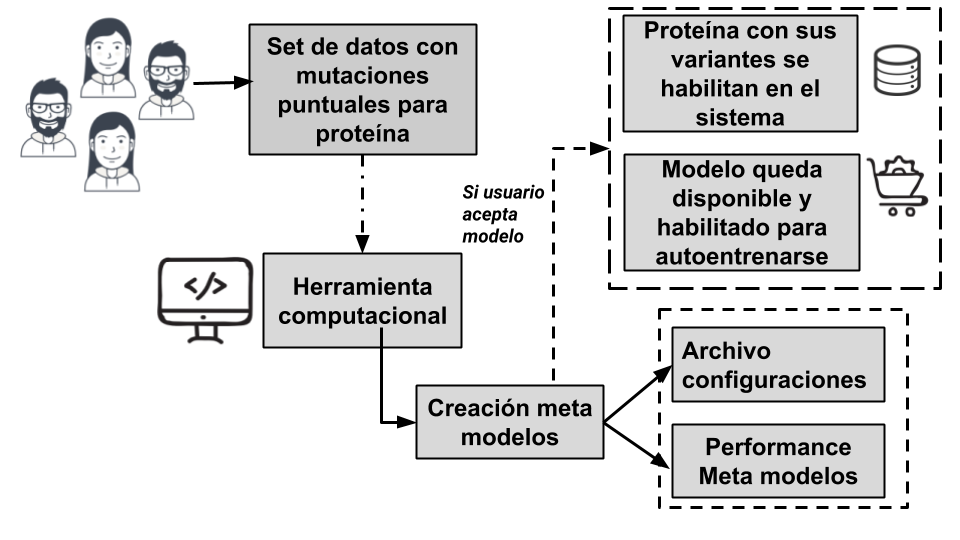
\includegraphics[scale=.4]{m3.png}
	\caption{Esquema representativo de flujo asociado a la herramienta de generación de meta modelos para mutaciones puntuales en proteínas de interés.}
	\label{C2:M3}
\end{figure}

La idea general, consiste en que usuarios de la herramienta, puedan entrenar sus propios modelos de clasificación o regresión, basados en la metodología expuesta en los pasos anteriores mediante el uso de Meta Learning Sytem Tools (Paper en Redacción). Para ello, los usuarios deben entregar sus set de datos con la información necesaria para ser procesada: cadena, residuo original, posición, residuo mutado y respuesta o efecto de la mutación, además del archivo PDB a ser procesado. La herramienta, aplica los pasos expuestos en la metodología de este capítulo generando un meta modelo basado en algoritmos de aprendizaje supervisado y las medidas de desempeño que permiten evaluar el modelo obtenido. Si el usuario acepta la metodología y por medio de un consentimiento informado, permite la publicación de los datos, el sistema habilita el acceso tanto a los meta modelos como a los set de datos y los agrega a la lista de procesos de modelos auto entrenables. Esto último, implica que ante la adición de nuevos ejemplos al set de datos, el sistema actualiza los modelos y las medidas de desempeño, aplicando la metodología expuesta, así, constantemente mantiene la actualización de la información y permite mantener en constante crecimiento los datos que contemplan el desarrollo de los modelos.

\section{Análisis y evaluación de los set de datos a utilizar}

A continuación, se exponen los resultados obtenidos hasta el momento y discusiones a cerca del proceso generado, contemplando desde la etapa inicial asociada a la búsqueda de set de datos de mutaciones en proteínas, la preparación de estos para la aplicación de la metodología desarrollada y la evaluación del funcionamiento de estos con el fin de generar meta modelos asociados a sistemas de mutaciones en proteínas y permitir el desarrollo de herramientas computacionales que faciliten dichas acciones. Adicional a esto, se expone un caso de estudio donde se emplea esta metodología para el desarrollo de modelos de clasificación de relevancia clínica de mutaciones asociadas a la enfermedad de von Hippel-Lindau, exponiendo las necesidades de adición de información en set de datos altamente no lineales.

\subsection{Set de datos utilizados}

En el presente apartado se describen las características básicas de los set de datos trabajados, así como también, qué representan las proteínas bajo las cuales se están desarrollando los modelos de estimadores.

\subsubsection{Descripción general}

Los set de datos utilizados, tanto para la formación de los inputs asociados al sistema, así como también la validación de respuesta correspondiente a la mutación que estos tienen, fueron extraídos desde distintas bases de datos de mutaciones en proteínas de estudios relacionados a los cambios que provoca la sustitución del residuo inicial, ya sea a nivel de cambios energéticos o estabilidad de la proteína.

11 set de datos con respuesta continua fueron obtenidos. Cada set de datos contemplaba como elemento a predecir, las diferencias de energía libre de Gibbs, entre los residuos originales y mutados. Las mutaciones fueron seleccionadas desdes diversos estudios en los cuales se reportaron, centrándose en \cite{Wainreb2011, Sun2017, petukh2016saambe, Alexov2012,prot20185}.

Adicional a los set de datos con respuesta continua, 8 conjuntos de elementos asociados a tareas de clasificación fueron obtenidos desde diversos estudios reportados a la actualidad \cite{ancien2018prediction, broom2017computational, capriotti2008three, quan2016strum, Capriotti2005, 1gzp030, Khan2010, masso2008accurate, getov2016saafec}. 

De tal manera, se generó un total de 19 conjuntos de set de datos, con respuesta categórica y continua, los cuales se asocian a proteínas independientes, usadas para la evaluación de las metodologías planteadas. Estas 19 proteínas junto con su descripción, se exponen en la Tabla \ref{cap2:tab2}.


\begin{longtable}[c]{|l|l|l|l|l|}
	\hline
	\multicolumn{5}{|c|}{\textbf{Resumen set de datos de proteínas y sus características}}                                                                                                                                                                                             \\ \hline
	\endfirsthead
	%
	\endhead
	%
	\textbf{\#} & \textbf{Código PDB} & \textbf{Tipo} & \textbf{Ejemplos} & \textbf{Descripción}                                                                                                                                                                                       \\ \hline
	1.          & 1A22                & Regresión     & 132               & \begin{tabular}[c]{@{}l@{}}Human growth hormone bound to single\\ receptor\end{tabular}                                                                                                                    \\ \hline
	2.          & 1CH0                & Regresión     & 191               & \begin{tabular}[c]{@{}l@{}}Crystal and molecular structures of the complex\\ of alpha-*Chymotrypsin with its inhibitor Turkey\\ Ovomucoid third domain\end{tabular}                                        \\ \hline
	3.          & 1DKT                & Regresión     & 119               & \begin{tabular}[c]{@{}l@{}}CKSHS1: Human cyclin dependent\\ kinase subunit, type 1 complex with\\ metavanadate\end{tabular}                                                                                \\ \hline
	4.          & 1FKJ                & Regresión     & 219               & \begin{tabular}[c]{@{}l@{}}Atomic structure of FKBP12-FK506, \\ an immunophilin  immunosupressant\\ complex\end{tabular}                                                                                   \\ \hline
	5.          & 1FTG                & Regresión     & 203               & \begin{tabular}[c]{@{}l@{}}Structure of apoflavodoxin: closure of\\ a Tyr/Trp aromatic gate leads to a\\ compact fold\end{tabular}                                                                         \\ \hline
	6.          & 1PPF                & Regresión     & 190               & \begin{tabular}[c]{@{}l@{}}X-Ray crystal structure of the complex\\ of human leukocyte elastase and the\\ third domain of the Turkey ovomucoid\\ inhibitor\end{tabular}                                    \\ \hline
	7.          & 1RX4                & Regresión     & 556               & \begin{tabular}[c]{@{}l@{}}Dihydrofolate reductase (E.C.1.5.1.3) complexed\\ with 5,10-Dideazatetrahydrofolate and\\ 2'-Monophosphadenosine 5'-Diphosphoribose\end{tabular}                                \\ \hline
	8.          & 1WQ5                & Regresión     & 239               & \begin{tabular}[c]{@{}l@{}}Crystal structure of tryptophan synthase\\ alpha-subunit from Escherichia coli\end{tabular}                                                                                     \\ \hline
	9.          & 2AFG                & Regresión     & 134               & Human acidic fibroblast growth factor                                                                                                                                                                      \\ \hline
	10.         & 3SGB                & Regresión     & 191               & \begin{tabular}[c]{@{}l@{}}Structure of the complex of Streptomyces\\ Griseus protease B and the Third domain\\ of the Turkey ovomucoid inhibitor\end{tabular}                                             \\ \hline
	11.         & 5AZU                & Regresión     & 203               & \begin{tabular}[c]{@{}l@{}}Crystal structure analysis of oxidize\\ Pseudomonas Aeruginoa Azurin at PH 5.5\\ and PH 9.0. A PH-induced conformational\\ Transition involves a peptide bond flip\end{tabular} \\ \hline
	12.         & 1BN1                & Clasificación & 1802              & Carbonic anhydrase II inhibitor                                                                                                                                                                            \\ \hline
	13.         & 1BVC                & Clasificación & 561               & \begin{tabular}[c]{@{}l@{}}Structure of a Biliverdin Apomyoglobin\\ complex\end{tabular}                                                                                                                   \\ \hline
	14.         & 1LZ1                & Clasificación & 848               & \begin{tabular}[c]{@{}l@{}}Human Lysozyme. Analysis of Non-Bonded\\ and Hydrogen-Bond interactions\end{tabular}                                                                                            \\ \hline
	15.         & 1STN                & Clasificación & 2193              & \begin{tabular}[c]{@{}l@{}}The crystal structure of Staphylococcal\\ Nuclease\end{tabular}                                                                                                                 \\ \hline
	16.         & 1VQB                & Clasificación & 820              & \begin{tabular}[c]{@{}l@{}}Gene V Protein (Single-Stranded DNA\\ Binding Protein)\end{tabular}                                                                                                             \\ \hline
	17.         & 2CI2                & Clasificación & 741               & \begin{tabular}[c]{@{}l@{}}Crystal and molecular structure of the\\ Serine proteinase inhibitor CI-2 from\\ Barley seeds\end{tabular}                                                                      \\ \hline
	18.         & 2LZM                & Clasificación & 2336              & Structure of Baceriophage T4 Lysosyme                                                                                                                                                                      \\ \hline
	19.         & 2RN2                & Clasificación & 712               & \begin{tabular}[c]{@{}l@{}}Structural details of ribonuclease H from\\ Escherichia Coli\end{tabular}                                                                                                       \\ \hline
	\caption{Resumen de proteínas utilizadas para el desarrollo de meta modelos basados en metodología Meta Learning System propuesta durante este capítulo.}
	\label{cap2:tab2}\\
\end{longtable}

Cada una de las proteínas presentan diferentes características y funcionalidades, algunas facilitan la unión a DNA, mientras que otras presentan propiedades enzimáticas, por otro lado, existen enzimas que representan inhibidores, entre las principales. Esto es interesante a la hora de evaluar el poder que presenta la metodología con respecto al análisis de diferentes proteínas, estructuras y complejos, ya que se presenta una gran variedad en cuanto a forma y funcionalidad de éstas, lo que implica que el sistema no se limita por cierto tipo de estructuras o complejos.

A modo de ilustrar las diferencias estructurales de las proteínas en estudio, en la Figura \ref{fig:proteins} se exponen algunas de las estructuras asociadas a las proteínas utilizadas para desarrollar modelos de clasificación o regresión.

\begin{figure}
	\centering
	\begin{subfigure}{0.4\textwidth}
		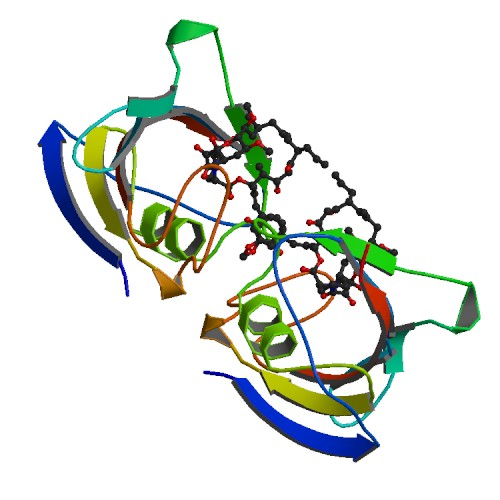
\includegraphics[width=\textwidth]{1fkj.jpg}
		\caption{1FKJ}
		\label{fig:1FKJ}
	\end{subfigure}
	~ %add desired spacing between images, e. g. ~, \quad, \qquad, \hfill etc. 
	%(or a blank line to force the subfigure onto a new line)
	\begin{subfigure}{0.4\textwidth}
		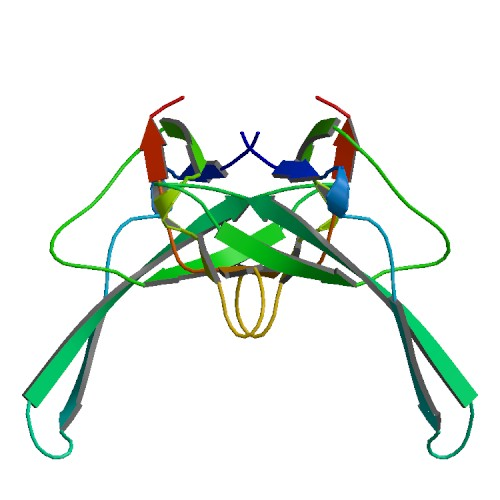
\includegraphics[width=\textwidth]{1vqb.jpg}
		\caption{1VQB}
		\label{fig:1VQB}
	\end{subfigure}
	~ %add desired spacing between images, e. g. ~, \quad, \qquad, \hfill etc. 
	%(or a blank line to force the subfigure onto a new line)
	\begin{subfigure}{0.4\textwidth}
		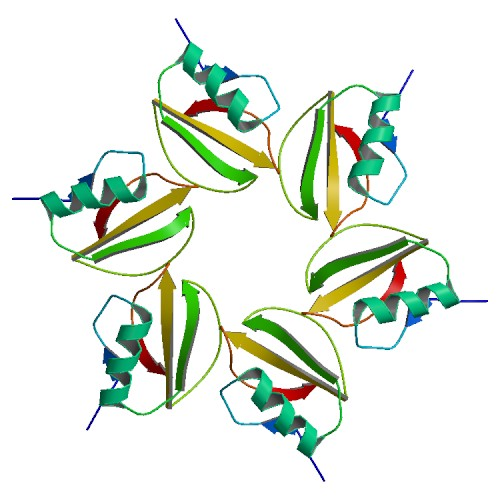
\includegraphics[width=\textwidth]{2ci2.jpg}
		\caption{2CI2}
		\label{fig:2CI2}
	\end{subfigure}
	
	\begin{subfigure}{0.4\textwidth}
		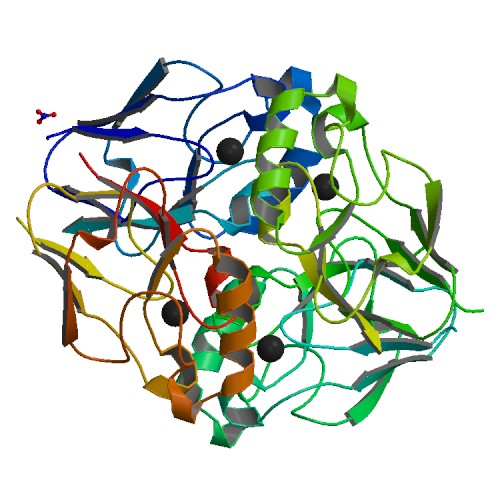
\includegraphics[width=\textwidth]{5azu.jpg}
		\caption{5AZU}
		\label{fig:5AZU}
	\end{subfigure}
	\caption{Representación de estructuras de proteínas ejemplos utilizadas para el desarrollo de meta modelos de clasificación.}
	\label{fig:proteins}
\end{figure}

Las mutaciones fueron recolectadas desde diferentes set de datos, por lo que, en caso de información ambigua, es decir, una misma mutación con diferentes respuestas, no fueron consideradas. Por otro lado, debido a que para la aplicación de la herramienta SDM se necesitaba la cadena a la cual pertenece en residuo, scripts desarrollados en Python y utilizando la librería BioPython, permitieron procesar los archivos asociados a las estructuras de las proteínas, identificadas desde el Protein Data Bank (PDB) \cite{abola1984protein}. Descartando aquellas mutaciones reportadas en las que no se encontró la cadena, obteniendo como resultante la cantidad de mutaciones reportadas para cada proteína expuestas en la Tabla \ref{cap2:tab2}.

\subsubsection{Evaluación del desbalance de clases y distribución de respuestas continuas}

El desbalance de clases se evaluó en aquellos set de datos con respuesta categórica, lo cual contempla, tres posibles casos: Neutral, Estable, No Estable, esto es debido a que todos los estudios donde se evalúan mutaciones, normalmente se analizan cambios que alteren la estabilidad de la proteína. En la Figura \ref{fig:desbalance}, se aprecia a modo ejemplo dos set datos y su distribución de categorías para la variable respuesta.

\begin{figure}[!h]
	\centering
	\begin{subfigure}{0.8\textwidth}
		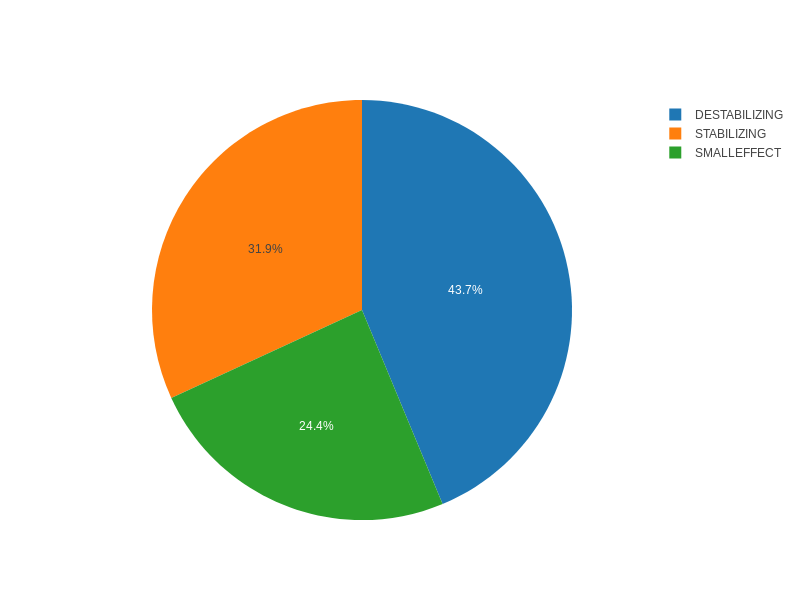
\includegraphics[width=\textwidth]{class1STN.png}
		\caption{1STN}
		\label{fig:des1}
	\end{subfigure}
	~ %add desired spacing between images, e. g. ~, \quad, \qquad, \hfill etc. 
	%(or a blank line to force the subfigure onto a new line)
	\begin{subfigure}{0.8\textwidth}
		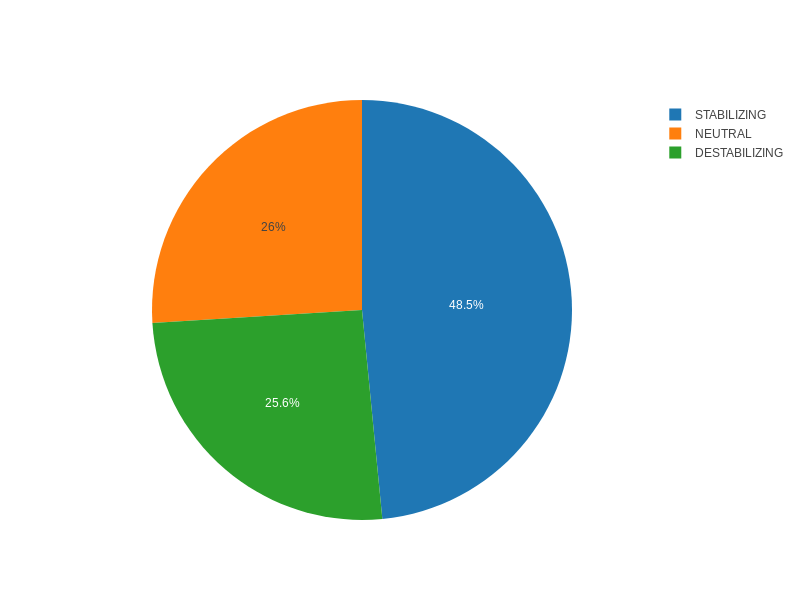
\includegraphics[width=\textwidth]{class2RN2.png}
		\caption{2RN2}
		\label{fig:des2}
	\end{subfigure}
	
	\caption{Evaluación del desbalance de clases en proteínas ejemplo.}
	\label{fig:desbalance}
\end{figure}

En las 8 proteínas en estudio para modelos de clasificación, la distribución de las categorías es similar a lo expuesta en la Figura \ref{fig:desbalance} para todas ellas, donde cerca del 50\% corresponden a mutaciones que afectan positivamente a la estabilidad, mientras que mutaciones que provocan cambios negativos o no generan diferencias, se encuentran en proporciones similares, ambas cercanas al 25\%. Si bien las proporciones son dispares, para este caso, se considera un desbalance como un elemento que representa menos de un 5\% del total de la muestra, además, dado a que la cantidad de ejemplos son elevadas, un 20\% o un 25\% implica cerca de 200 mutaciones, en promedio, que cumplen dicha característica. Además, el hecho de que exista una cantidad inferior de mutaciones no benéficas a la estabilidad viene dada a la dificultad de encontrar y reportar mutaciones que afecten negativamente a la para una proteína dado a la propensión filogenética \cite{Olivera-Nappa2011} que estos ocurran, lo cual se ve reflejado en las diferencias asociadas a cambios positivos dentro del set de mutaciones. No obstante, si bien el hecho de que la propensión filogenética indique que el cambio tiende a mejorar estabilidad, diseñar mutantes con mejoras en propiedades de interés, es un problema latente en la actualidad, de alto costo económico y computacional y con una gran demanda desde diferentes áreas del conocimiento.|

En los set de datos para el desarrollo de modelos de regresión, se evaluó la distribución de la respuesta, en este caso, valores de $\Delta\Delta\ G$ asociado a diferencias de energía libre producidas entre el residuo mutado y el original, tal que: $\Delta\ Res_{mut}\ - \Delta\ Res_{wild}\ = \Delta\Delta\ G$. 

Las distribuciones se evaluaron utilizando el test de Shapiro, con el fin de determinar si la distribución se comportaba como una normal. Para todas las proteínas estudiadas, en los 11 set de datos, las respuestas presentaron distribución normal, con valores de Shapiro sobre 0.8 y un p-value $\leq$ 0.01, lo cual indica una alta confianza estadística en los resultados presentados por dicho test.

Una visualización de las distribuciones puede generarse a partir del desarrollo de histogramas, los cuales, a modo de ejemplo se expone en la Figura \ref{fig:histogram}.

\begin{figure}[!h]
	\centering
	\begin{subfigure}{0.48\textwidth}
		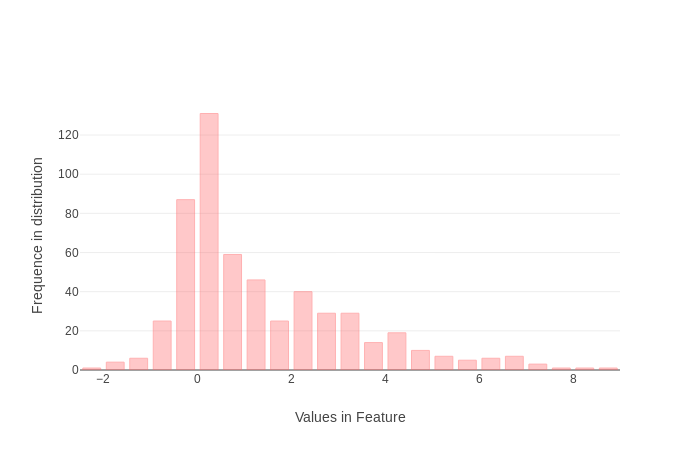
\includegraphics[width=\textwidth]{1RX4.png}
		\caption{Histograma para respuesta continua en 1RX4}
		\label{fig:hist1}
	\end{subfigure}
	~ %add desired spacing between images, e. g. ~, \quad, \qquad, \hfill etc. 
	%(or a blank line to force the subfigure onto a new line)
	\begin{subfigure}{0.48\textwidth}
		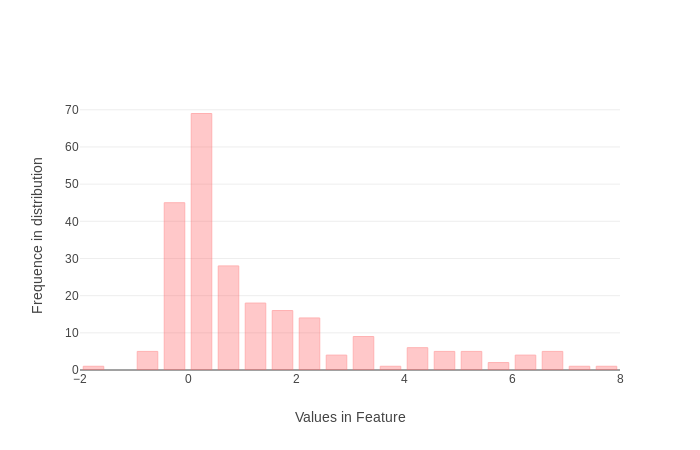
\includegraphics[width=\textwidth]{1WQ5.png}
		\caption{Histograma para respuesta continua en 1WQ5}
		\label{fig:hist2}
	\end{subfigure}
	
	\caption{Evaluación de la distribución de respuesta continua en set de datos de proteínas.}
	\label{fig:histogram}
\end{figure}

El análisis de estas características es relevante a la hora de diseñar modelos de clasificación o regresión, debido a que si existe una tendencia por una clase condiciona al clasificador a \textit{"aprender en base a la mayoría"}, por lo que puede aumentar los errores en cuanto a falsos positivos, dado a que, no se tiene la cantidad de ejemplos suficientes para una clase que permitan al modelo capturar las posibles variaciones asociadas a ésta.

Dado a los análisis de evaluación de representatividad de categorías en el set de datos y distribución de respuestas continuas, se expone que los set de datos seleccionados no presentan desbalance significativo para el caso de desarrollo de modelos de clasificación y a su vez, todas las respuestas asociadas a cambios en la energía libre para modelos de regresión, presentan distribución normal. Razón por la cual, es factible el desarrollo de modelos asociados a las respuestas presenten en los set de datos seleccionados. No obstante, sólo se ha considerado el problema del desbalance y la evaluación de distribución en la respuesta continua, una vez caracterizado los set de datos a partir de las propiedades fisicoquímicas y termodinámicas, se analizarán las características y cómo éstas condicionan la clasificación o la predicción de cambios energéticos.
